\documentclass[10pt]{article}
\usepackage{mathtools}
\usepackage{graphicx}
\usepackage{amsmath}
\usepackage{amsfonts}
\usepackage{microtype}
\usepackage{hyperref}
\usepackage{tikz-cd}
\usepackage{amssymb}
\usepackage{comment}
\usepackage{mymacros}
\usepackage{caption}
\usepackage{subcaption}

\setlength{\parindent}{0cm} 
\setlength{\parskip}{1em}

\graphicspath{{./img/}}

\begin{document}
\begin{center}
  \huge \textbf{Project 1}
\end{center}
\section{Introduction}
In this project we study the one-dimentional Poisson equation 
with Dirichlet boundary conditions which reads 

\begin{equation*}
 -u''(x)=f(x),\quad x\in (0,1),\quad u(0)=u(1)=0.
\end{equation*}

In order to model this equation in a computer we need to define the 
discretized approximated solution to $ u(x) $ as $v_i=v(x_i) $ where
 $x_i=x_0+ih=ih$ since $x_0=0$. We let $x_{n+1}=1$, this means $h=\frac{1}{n+1}$.
 From Taylor expanding $u(x\pm h)$ we get 
 $$u(x\pm h)=u(x)\pm hu'(x)+\frac{h^2}{2!}u''(x)\pm O(h^3)$$
We see that $u''(x)=\frac{u(x+h)+u(x-h)-2u(x)}{h^2}-O(h^4)$. Hence for the approximated solution
 we get that $$-\frac{v_{i+1}+v_{i-1}-2v_i}{h^2}=f_i\quad \text{for i}=1,...,n$$ where $f_i=f(x_i)$. 
 If we set $g_i=h^2f_i$ we get that $2v_i-v_{i+1}-v_{i-1}=g_i$. 
 This is just $n$ equations, given by $i=i,...,n$. We can write this in matrix form 
 $$\mathbf{A}\mathbf{v}=\mathbf{g}, $$ where $\mathbf{A}$ is a $n\times n$ 
 tridiagonal matrix on the form $$\mathbf{A}=\begin{bmatrix}
   2 & -1 & 0 & \dots & ... & 0 \\
   -1 & 2 & -1 & 0 & ... & 0 \\
   0  & -1 & 2 & -1 & 0 & ... \\
   \vdots & 0 & \ddots & \ddots & \ddots & ...\\
   0 & ... & ... & -1 & 2 & -1\\
   0 & ... & ... & 0 & -1 & 2 
 \end{bmatrix}$$

 $\mathbf{v}$ and $\mathbf{g}$ are vectors on the form 
 $$\mathbf{v}=\begin{bmatrix}
   v_1\\v_2\\\vdots\\v_n
 \end{bmatrix}
 \qquad
 \mathbf{g}=\begin{bmatrix}
   g_1\\g_2\\\vdots\\g_n
 \end{bmatrix}
 $$
We will use the source term $f(x)=100e^{-10x}$, this gives the particular solution 
$u(x)=1-(1-e^{-10})x-e^{-10x}$. This is easy to see since $-e^{-10x}$ is the general solution,
 hence $-u''(x)=f(x)$, and $u(0)=u(1)=0$ is trivial. 

 \section{General algorithm}
 The general algorithm to solve a set of equation on a tridiagonal form is done by a forward and backward substitution. On matrix form the problem is $\mathbf{A}\mathbf{v}=\mathbf{g}$. Where 
 $$
 \mathbf{A}=  \begin{bmatrix}
  2 & -1 & 0 & \dots & ... & 0 \\
  -1 & 2 & -1 & 0 & ... & 0 \\
  0  & -1 & 2 & -1 & 0 & ... \\
  \vdots & 0 & \ddots & \ddots & \ddots & ...\\
  0 & ... & ... & -1 & 2 & -1\\
  0 & ... & ... & 0 & -1 & 2 
 \end{bmatrix}
 $$


 \begin{figure}[h]
  \begin{subfigure}{.5\textwidth}
    \centering 
    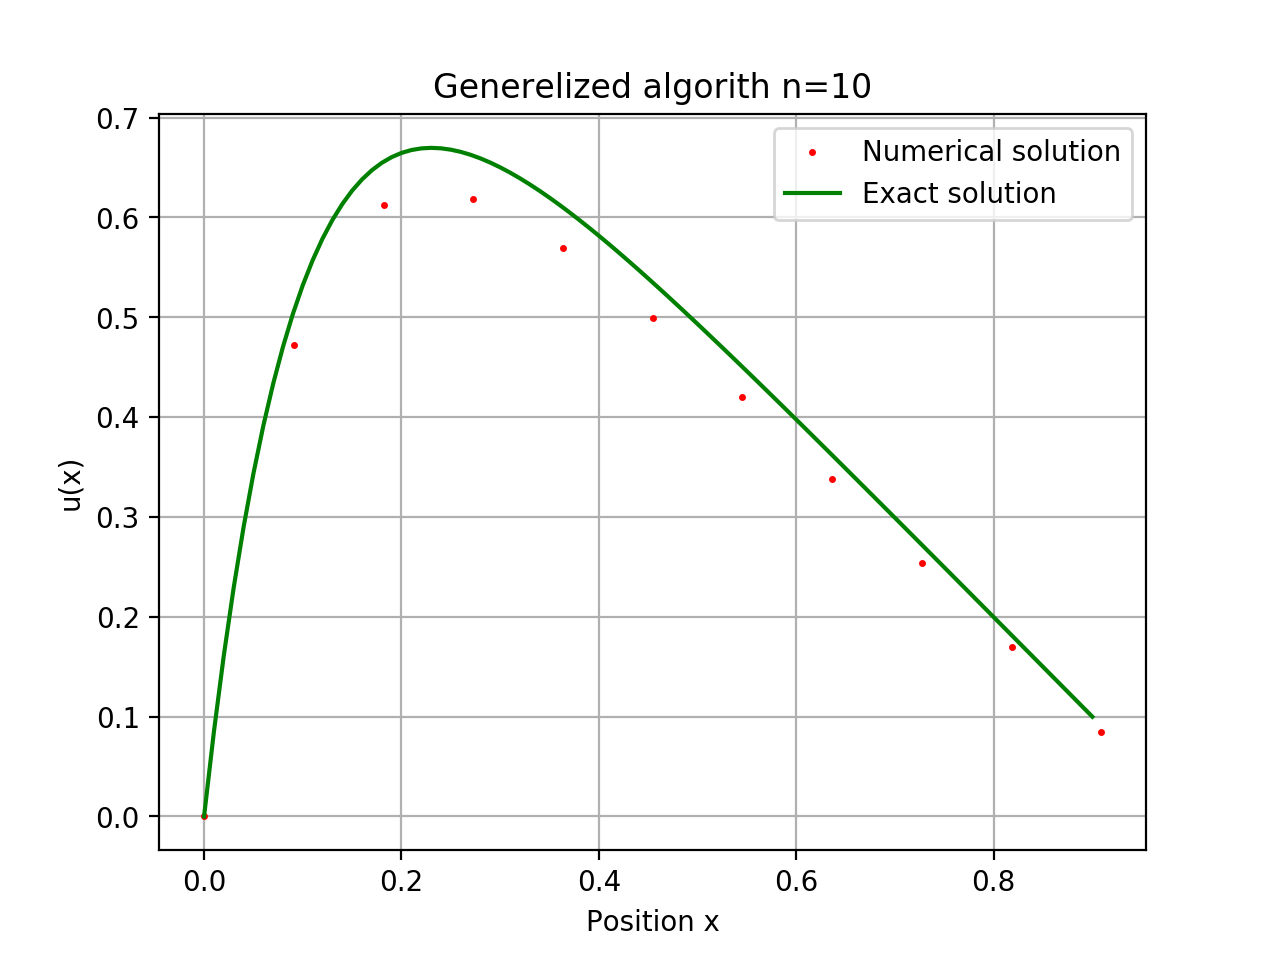
\includegraphics[scale=0.4]{alg-0-n10plot.png}
    \caption{Test}
    \label{fig:sub1}
  \end{subfigure}
  \begin{subfigure}{.5\textwidth}
    \centering
    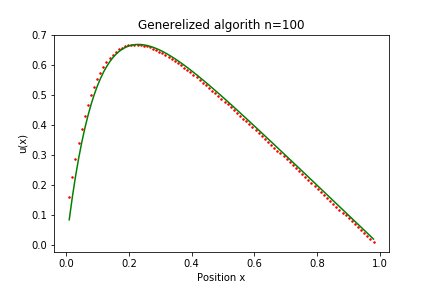
\includegraphics[scale=0.4]{alg-0-n100plot.png}
    \caption{Test 1}
  \end{subfigure}
  \begin{subfigure}{.5\textwidth}
    \centering
    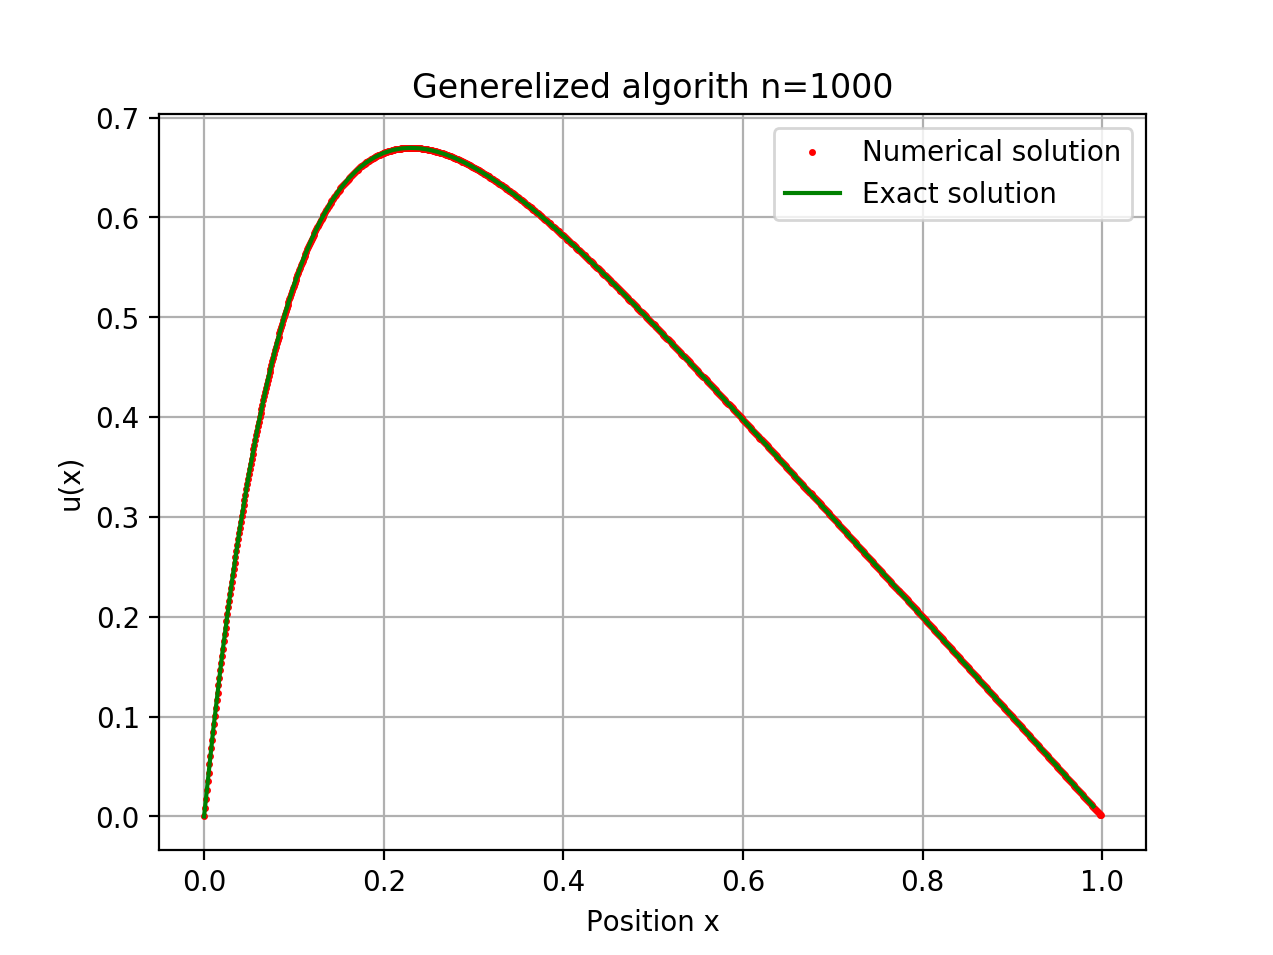
\includegraphics[scale=0.4]{alg-0-n1000plot.png}
    \caption{Test 2}
  \end{subfigure}
    

\end{figure}


\end{document}